\scanpage{9}
\mspage{652}

is a \uline{nilpotent} endomorphism of $M_K$.
thus an element \deleted{of $\operatorname{End}(M)\otimes_A K$}
\[
(8)\qquad X\in\operatorname{End}_A(M)\otimes_A K,\qquad X^n=0.
\]
($A$ the affine ring of $S$, which is a \deleted{\illegible{1}} gauge)
We shall have by hypothesis
\[
g_\eta=\varphi_\eta(1)=\sum\frac{X^i}{i!}\in
\diagram{\begin{tikzcd}[ampersand replacement=\&,row sep=1.6em]
\operatorname{Aut}(M)\arrow[d,phantom,"\cap" description]\\
\operatorname{Aut}(M_K)
\end{tikzcd}}
\]
i.e.
\[
(9)\qquad \sum\frac{X^i}{i!},\quad
\sum(-1)^i\frac{X^i}{i!}\in\operatorname{End}_A(M)
\]
and the question whether $\varphi_\eta$ comes from a homomorphism of groups
$\mathbb G_a\longrightarrow G$ comes down to that of knowing whether
\[
(10)\qquad \frac{X^i}{i!}\in\operatorname{End}_A(M)
\qquad\forall\,\unsure{(1\le i\le n-1)|1\le i\le n-1}
\]
\margin{(for $i=0$ and $\unsure{i\ge n|i=n}$ this is trivial)}

For $n=2$ this is trivial, For $n=3$ \uline{\unsure{ditto|ditto}}
(in (9) there is a single term with a denominator).
\[
\deleted{\varphi_\eta(\lambda)=1+X\lambda+\frac{X^2}{2}\lambda^2
\qquad\left\{\begin{array}{l}X\in M_3(K)\\X^3=0\end{array}\right.}
\]
the first \unsure{doubtful} case is $n=4$
\deleted{and the question is to know whether}
\[
\varphi_\eta(\lambda)=1+X\lambda+\frac{X^2}{2}\lambda^2+
\frac{X^3}{6}\lambda^3
\qquad\begin{array}{l}X\in M_4(K)\\X^4=0\end{array}
\]
we have by hypothesis $\varphi_\eta(1)$ and $\varphi_\eta(-1)$ in $M_4(A)$,
i.e.
\[
(11)\qquad \frac{X^2}{2}\mathbin{\pm}\frac{X^3}{6}\in M_4(A)
\]
we wonder whether it follows that
\[
(12)\qquad \frac{X^2}{2},\frac{X^3}{6}\in M_4(A)\qquad ?
\]
If $2$ invertible in $A$ this is clear, for we deduce from (11) that $X^2\in M_4(A)$
hence $\dfrac{X^2}{2}\in M_4(A)$, hence also $X^3/6\in M_4(A)$, OK.
Thus the difficulty
\margin{8}

% Pied de page imprimé de l'archive.
\begin{center}
\small
8\\
\texttt{https://grothendieck.umontpellier.fr}\\
Université de Montpellier, UMR CNRS 5149, Case courrier 051, Place Eugène Bataillon\\
34095 Montpellier cedex 5 - France
\end{center}

\scanpage{10}
arises here in residual characteristic 2. \deleted{\unsure{Let}} Suppose \deleted{\unsure{$\pi$}} \inserted{for simplicity that 2 is} a \unsure{uniformizer} $\unsure{\pi}$ of $A$, we shall have, if $X\notin M_4(A)$
\[
X=\frac{1}{\unsure{\deleted{\pi}\inserted{2}}^{\nu}}X_0
\quad\text{with}\quad
\begin{gathered}
X_0\in M_4(A)\ \deleted{\unsure{\pi M_4}}\\
X_0\notin \unsure{\deleted{\pi}\inserted{2}}M_4(A)
\end{gathered}
\]
hence \deleted{\unsure{and the}} the datum of $X$ is equivalent to that of
\[
X_0\unsure{=|\in}\deleted{\illegible{1}}(a_{ij})_{1\leq i,j\leq4},\quad
\deleted{\unsure{\in M_4(A)|\in A}}\quad\text{the }a_{ij}\in A\text{ not all}
\]
divisible by 2, with \deleted{$\unsure{X_0^4}$}.
\[
(11\,\text{bis})\qquad X_0^4=0,\qquad
\frac12\frac{X_0^2}{2^{2\nu}}\pm\frac16\frac{X_0^3}{2^{3\nu}}\in M_4(A)
\]
--- and the question is whether it follows that we \unsure{have|have}
\[
(12\,\text{bis})\qquad
\frac12\frac{X_0^2}{2^{2\nu}},\frac12\frac{X_0^3}{2^{3\nu}}\in M_4(A)\qquad ?
\]

Of\deleted{\illegible{1}} course, the \deleted{\unsure{q}} answer is \unsure{trivially|totally} yes, if $X_0^3=0$ \inserted{i.e. $X^3=0$} --- so we are interested in the case where $X_0^3\ne0$, i.e. \deleted{$\unsure{X_{0\eta}}$} $g_\eta$ is ``principal unipotent.

\margin{\uline{Attempt at a characterization of quasi-\deleted{\illegible{1}}unipotent sections}}
2.\quad To get to the bottom of it, one would need a counterexample in the preceding context (with a nilpotent matrix of order 4) --- or a theorem ! But for my purpose, it seems that it is not essential to have a solution of this problem.

On the other hand, I shall try the

\uline{Theorem} (!) Let $G$ be a group scheme \inserted{(separated)} locally of finite presentation over a scheme $S$\deleted{\illegible{1}} which is quasi-compact, and let $g$ be a section of $G$. For $g$ to be quasi-unipotent, it
\margin{9}

% Pied de page imprimé de l'archive.
\begin{center}
\small
9\\
\texttt{https://grothendieck.umontpellier.fr}\\
Université de Montpellier, UMR CNRS 5149, Case courrier 051, Place Eugène Bataillon\\
34095 Montpellier cedex 5 - France
\end{center}

\scanpage{11}
\mspage{653}
\margin{\figure{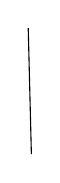
\begin{tikzpicture}[x=1cm,y=1cm]\draw (0,0)--(-0.04,1.6);\end{tikzpicture}}}
is necessary and sufficient that there exist an integer $n>0$, and a homomorphism of group schemes $\varphi:\mathbb G_a\longrightarrow G$, such that we have
\[
(13)\qquad \varphi(1)=g^n.
\]

Sufficiency being trivial, it is a matter of examining necessity. For simplicity, we shall again suppose $S$ noetherian and integral --- once $S$ is assumed noetherian, I think that the reduction to the integral case should be done by easy dévissages, which I do not feel like doing, for lack of essential need ! I shall therefore examine the case $S$ noetherian integral, generic point $\eta$

a) Characteristic \unsure{of} $\eta$ is $>0$. Then \deleted{$\unsure{g_\eta}$} the hypothesis on $g_\eta$ is that $g_\eta$ is of finite order --- hence $\exists n>0$ such that $g_\eta^n=1$, hence $g^n=1$. We shall take in (13) this $n$, and $\varphi$ the trivial homomorphism.

b) Case where $\eta$ of characteristic zero. Let $\varphi$
\[
(14)\qquad \varphi_{1\eta}:\mathbb G_{a\eta}\longrightarrow G_\eta
\]
be defined by the condition
\[
g_\eta=\varphi_{1\eta}(1)
\]
let $U_1$ be its ``open set of definition'' in $S$.

Let
\[
\varphi_{n\eta}(\lambda)=\lambda^n=\varphi_{1\eta}(n\lambda):\mathbb G_{a\eta}\longrightarrow G_\eta
\]
and let $U_n$ be its open set of definition. We thus have
\[
(15)\qquad\varphi_{n\eta}(1)=g^n\quad\text{on }U_n
\]
\margin{10}

% Pied de page imprimé de l'archive.
\begin{center}
\small
10\\
\texttt{https://grothendieck.umontpellier.fr}\\
Université de Montpellier, UMR CNRS 5149, Case courrier 051, Place Eugène Bataillon\\
34095 Montpellier cedex 5 - France
\end{center}

\scanpage{12}
\deleted{\mspage{653}}
and
\[
(16)\qquad n\mid n'\quad\Longrightarrow\quad U_n\subset U_{n'}.
\]
We must prove that the union of the $U_n$ is $S$. We are reduced to the case $S$ local, and where $\varphi_1$ is already defined in
\[
(17)\qquad U_1=S\setminus\{s\},\qquad s\text{ the closed point of }S
\]
and this comes down to the

\margin{\unsure{to}}
\uline{Lemma} (!) \unsure{Let} $S$ be noetherian integral, $G$ a group scheme \inserted{separated} locally of finite presentation over $S$, $U$ a nonempty open set of $S$, $\varphi_U:\mathbb G_{aU}\longrightarrow G_U$ a homomorphism of groups, we assume that $\varphi_U(1)=g_U$ extends to a section $g$ of $G$ over all of $S$ (\unsure{necessaril\textsuperscript{y}} unipotent, by known general results \unsure{of|of the} SGA 3) Then there exists an integer $>0$ such that $\varphi_U^n:\lambda\longmapsto\varphi_U(\lambda^n)$ extends \unsure{to|over} $S$ a homomorphism
\[
\varphi_n:\mathbb G_a\longrightarrow G.
\]

I am not going to try to prove it in this general context of general group schemes, and shall restrict myself, as a decisive test (to carry conviction that \unsure{it works}) the case where $G=\mathrm{Gl}(n)_S$, as earlier, and that where $S$ moreover is regular of dimension 1.

Thus we are reduced to the situation of a \unsure{gauge} $A$, and of $X\in M_n(K)$ ($K$ the field of fractions) satisfying
\margin{11}

% Pied de page imprimé de l'archive.
\begin{center}
\small
11\\
\texttt{https://grothendieck.umontpellier.fr}\\
Université de Montpellier, UMR CNRS 5149, Case courrier 051, Place Eugène Bataillon\\
34095 Montpellier cedex 5 - France
\end{center}

\scanpage{13}
\mspage{\textcircled{654}}
\[
(18)\qquad
\left\{\begin{array}{l}
X\in M_n(K)\\
X^n=0,\quad\displaystyle\sum\frac{X^i}{i!}\in M_n(A),\quad
\displaystyle\sum\frac{(-1)^iX^i}{i!}\in M_n(A)
\end{array}\right.
\]
and we want to show that there exists an integer $d>0$ such that we have
\[
(19)\qquad\frac{d^iX^i}{i!}\in M_n(A)\qquad(1\leq i\leq n-1)
\]
If $A$ is of characteristic 0 i.e. if it is a $\mathbb Q$-algebra, this \deleted{implies} \inserted{is equivalent} moreover :
\[
\frac{X^{\deleted{\unsure{i|0}}}}{\deleted{\unsure{i!}}}\in M_n(A)
\qquad\deleted{\text{\illegible{1}}\ X^i\in M_n(A))}
\]
\margin{\figure{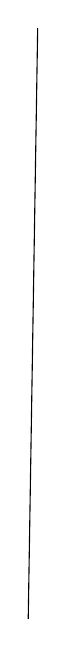
\begin{tikzpicture}[x=1cm,y=1cm]\draw (0,0)--(0.12,7.5);\end{tikzpicture}}}
\margin{the case of characteristic zero is settled in the affirmative by means of the logarithm function --- setting
\[
X+\frac{X^2}{2!}+\cdots+\frac{X^{n-1}}{(n-1)!}=Y,
\]
we shall have
\[
\exp X=1+Y,\quad\text{hence}
\]
\[
X=\log(1+Y)=Y-\frac{Y^2}{2}+\frac{Y^3}{3}\ldots
\]
Works over any base ring of characteristic zero\ldots}
\margin{$\unsure{b|0}$}
i.e. It would have to be that in the case of characteristic 0, it is $\varphi_U$ itself that can already extend to all of $S$. The first doubtful case in this regard seems to me $\unsure{n|m}=5$
\[
(20)\qquad\left\{\begin{array}{l}
\deleted{\unsure{X^5=0}}\quad\inserted{X\in M_5(\unsure{A|K}),\ X^5=0}\\
\displaystyle\frac{X^2}{2}\pm\frac{X^3}{3!}+\frac{X^4}{\deleted{\unsure{2}}4!}\in M_5(A)\\[3pt]
\overset{?}{\Longrightarrow}\quad\deleted{\unsure{X^2,X^3,X^4}}\quad X\in M_5(A)
\end{array}\right.
\]

On the other hand, in the case considered \unsure{a little earlier} ($n=4$, residual characteristic 2 --- the only one that causes difficulties) it is clear that it suffices to take for $d$ a sufficiently large power of 2.

This remark applies to the mixed characteristic cases. We should indeed have this

\uline{Corollary to the lemma} \unsure{dubious} : if $S$ is local, of residual characteristic $p>0$, and if $\varphi$ is defined on an open set which contains $S-V(p)$, (i.e. if the complement of $U$ is of characteristic $p\unsure{>|\geq}0$ --- in fact unnecessary of course that $S$ be local) then $\exists q=p^{\unsure{r|n}}$ such that $\varphi^q$ extends.
\margin{12}

% Pied de page imprimé de l'archive.
\begin{center}
\small
12\\
\texttt{https://grothendieck.umontpellier.fr}\\
Université de Montpellier, UMR CNRS 5149, Case courrier 051, Place Eugène Bataillon\\
34095 Montpellier cedex 5 - France
\end{center}